\documentclass[conference, letterpaper, 10pt, times]{IEEEtran}

\usepackage[T1]{fontenc}
\usepackage{amsfonts}
\usepackage{amsmath}
\usepackage{amsthm}
\usepackage{bm}

\usepackage[dvipsnames]{xcolor}
\usepackage{graphicx}
\usepackage{tikz}
\usetikzlibrary{arrows.meta, calc, fit, positioning}

\usepackage[binary-units, per-mode=symbol]{siunitx}
\sisetup{detect-all, range-phrase=--, range-units=single}

\usepackage[basic]{complexity}
\usepackage[super,negative]{nth}

\usepackage[british]{babel}
\usepackage{csquotes}

\usepackage{booktabs}
\usepackage[
activate={true,nocompatibility},
final,
tracking=true,
%kerning=true,spacing=true
]{microtype}
\microtypecontext{spacing=nonfrench}

%% Fix indent in new section...
\newcommand{\subparagraph}{}
\usepackage{titlesec}
\titlespacing*{\section}{0pt}{1.5ex}{0.7ex}
\titlespacing*{\subsection}{0pt}{1.5ex}{0.7ex}
\titlespacing*{\paragraph}{0pt}{1.5ex}{0.7ex}
%\titleformat*{\filcenter\scshape}

\usepackage{enumitem}
\setlist[description]{leftmargin=8em,style=nextline}

%bib
\usepackage[style=ieee,maxnames=3,mincitenames=1,maxcitenames=2,maxbibnames=99,mincrossrefs=5,sortcites,backend=bibtex,uniquelist=false]{biblatex}
\addbibresource{papers-off.bib}
\addbibresource{confs-off.bib}
\addbibresource{books-off.bib}
\addbibresource{rfc.bib}
\addbibresource{misc.bib}

%picky abt et al.
%\usepackage{xpatch}

%\xpatchbibmacro{name:andothers}{%
%	\bibstring{andothers}%
%}{%
%	\bibstring[\emph]{andothers}%
%}{}{}

% emph'd et al. for ieee style
\DefineBibliographyStrings{english}{%
	andothers = {\emph{et al}\adddot}
}
\DeclareFieldFormat[inproceedings]{url}{}
\DeclareFieldFormat[article]{url}{}

%opening!

\newcommand{\mytitle}{Improving Direct-Control Reinforcement Learning for Network Intrusion Prevention}

\usepackage{url}
\usepackage{hyperref}
\usepackage{cleveref}
\newcommand{\crefrangeconjunction}{--}

\hypersetup{
	colorlinks,
	citecolor=black,
	filecolor=black,
	linkcolor=black,
	urlcolor=black,
	pdftitle={\mytitle{}},
	pdfauthor={Kyle A. Simpson, Dimitrios P. Pezaros}
}
\newcommand*{\email}[1]{\href{mailto:#1}{\nolinkurl{#1}} } 

\usepackage{titling}
\settowidth{\thanksmarkwidth}{*}
\setlength{\thanksmargin}{-\thanksmarkwidth}

%% Enable /thanks
\IEEEoverridecommandlockouts
\makeatletter
\def\footnoterule{\relax%
	\kern-5pt
	\hbox to \columnwidth{\hfill\vrule width 0.5\columnwidth height 0.4pt\hfill}
	\kern4.6pt}
\makeatother

% make math easy
\newcommand{\acval}[3]{\ensuremath{\operatorname{\hat{q}}(#1, #2, #3)}}
\newcommand{\wvec}[1]{\ensuremath{\bm{w}_{#1}}}

%thm environments
\newtheorem{thm}{Theorem}
\newtheorem{corr}{Corollary}[thm]

\makeatletter
\DeclareRobustCommand{\rvdots}{%
	\vbox{
		\baselineskip4\p@\lineskiplimit\z@
		\kern-\p@
		\hbox{.}\hbox{.}\hbox{.}
}}
\makeatother

% Official colours!

\definecolor{uofguniversityblue}{rgb}{0, 0.219608, 0.396078}

\definecolor{uofgheather}{rgb}{0.356863, 0.32549, 0.490196}
\definecolor{uofgaquamarine}{rgb}{0.603922, 0.72549, 0.678431}
\definecolor{uofgslate}{rgb}{0.309804, 0.34902, 0.380392}
\definecolor{uofgrose}{rgb}{0.823529, 0.470588, 0.709804}
\definecolor{uofgmocha}{rgb}{0.709804, 0.564706, 0.47451}

\definecolor{uofglawn}{rgb}{0.517647, 0.741176, 0}
\definecolor{uofgcobalt}{rgb}{0, 0.615686, 0.92549}
\definecolor{uofgturquoise}{rgb}{0, 0.709804, 0.819608}
\definecolor{uofgsunshine}{rgb}{1.0, 0.862745, 0.211765}
\definecolor{uofgpumpkin}{rgb}{1.0, 0.72549, 0.282353}
\definecolor{uofgthistle}{rgb}{0.584314, 0.070588, 0.447059}
\definecolor{uofgpillarbox}{rgb}{0.701961, 0.047059, 0}
\definecolor{uofglavendar}{rgb}{0.356863, 0.301961, 0.580392}

\definecolor{uofgsandstone}{rgb}{0.321569, 0.278431, 0.231373}
\definecolor{uofgforest}{rgb}{0, 0.317647, 0.2}
\definecolor{uofgburgundy}{rgb}{0.490196, 0.133333, 0.223529}
\definecolor{uofgrust}{rgb}{0.603922, 0.227451, 0.023529}

%-------------------------------------%
%-------------------------------------%

\title{\mytitle{}}
\author{
	Kyle A.\ Simpson\thanks{This work was supported by the Engineering and Physical Sciences Research Council [grant number EP/M508056/1].},
	Dimitrios P.\ Pezaros\\
	University of Glasgow, Glasgow, Scotland,\\
	\email{k.simpson.1@research.gla.ac.uk}
}

% Remove date, leave no spacing.
\predate{}
\postdate{}
\date{}

\begin{document}

%% If needed, make urls typewritery
%\urlstyle{tt}

\maketitle

\begin{abstract}
Network intrusion detection and prevention systems backed by machine learning (and the autonomous operation they promise) have been long-heralded, but face problems hampering effective deployment.
The detection problem in this domain is fraught with difficulty; it is an evolving, non-stationary problem as usage patterns shift, new protocols and applications are introduced, and is compounded by burstiness and seasonal variation.

\emph{Reinforcement learning} (RL) may overcome the detection problem for certain classes of anomaly by managing and monitoring \emph{consequences}; an agent's role is to learn to optimise performance criteria (which are always available).

We present...
?? Contribs

?? Taking up space to figure out how much room I have for an intro

?? still taking up space...

?? still going...

?? done...
\end{abstract}

\section{Introduction}

Network anomaly detection, intrusion detection and intrusion prevention are continually evolving problems, compounded by the partial, non-IID view of data at each point in the network.
Attacks and anomalous behaviours evolve, becoming more sophisticated or employing new vectors to harm a network or system's confidentiality, integrity, or availability without being detected.
These attacks and anomalies have measurable consequences and symptoms which allow a skilled analyst to infer new signatures for detection by misuse-based classifiers, but unseen attacks may only be defended against after-the-fact.
This issue is inherent to \emph{misuse-} or \emph{signature-based} intrusion detectors, and it has been long-hoped that \emph{anomaly-based} detectors would surpass this by making effective use of statistical measures.

While \emph{machine learning} (ML) approaches seem like a sensible fit for this problem, in \citeyear{DBLP:conf/sp/SommerP10} \textcite{DBLP:conf/sp/SommerP10} identified the `failure to launch' of ML-based anomaly detection systems---to quite a large extent, this remains the case today.
Their application is made difficult due to significant operational differences from standard ML tasks, alongside certain characteristics of network traffic.
Briefly, these are the diversity of network traffic across varying timescales \cite{DBLP:conf/sp/SommerP10} and significant burstiness \cite{DBLP:journals/ccr/LelandWTW95}.
Above the aggregate level, the constant deployment of new services and new protocols means that traffic is \emph{non-stationary} and displays an evolving notion of normality.
Further issues arise from the extraordinarily low tolerance for false positives inherent to network intrusion detection \cite{DBLP:conf/ccs/Axelsson99}, and the challenges encountered when learning from unlabelled (often partial) data.
All of these factors greatly inflate the difficulty of the detection problem.

For certain classes of problem like flooding-based DDoS attacks, \emph{reinforcement learning} (RL) offers another perspective.
The role of an RL agent differs from that of a standard classifier, adaptively reacting to threats by assuming the role of a feedback loop for network optimisation, typically to safeguard service guarantees.
In a sense, this allows us to ``overcome'' the difficulties of the detection problem by monitoring \emph{performance characteristics and consequences} in real-time; by looking for the effect rather than the cause.
The intent is to augment what existing misuse-based solutions can provide, by automatically alerting, recording and controlling what are believed to be illegal system states.
%Whether it takes direct control of the network, or is used indirectly to optimise a key part of another system, more powerful `deep' RL techniques (and well-founded action spaces) aren't yet well explored for network IDS/IPS.
%These range from more modern training algorithms \cite{DBLP:journals/corr/SchulmanWDRK17, DBLP:conf/icml/SchulmanLAJM15}, to evolutionary strategies \cite{DBLP:journals/corr/SalimansHCS17, DBLP:journals/corr/abs-1802-08842}, hierarchical action composition \cite{DBLP:journals/corr/abs-1710-09767}, and competitive multi-agent learning \cite{DBLP:journals/corr/abs-1710-03748}.

?? Reference to the possible mistreatment of RL in our domain? The problem of ``blind application'' so hated by \textcite{DBLP:conf/sp/SommerP10}.

This paper contributes:
\begin{itemize}
	\item A DDoS mitigation system based on direct-control reinforcement learning designed for deployment in real-world software-defined networks (\cref{sec:environment-and-rl-algorithm,sec:rethinking-the-state-space}).
	\item Important weaknesses and flaws in the past design and evaluation of similar techniques \cite{DBLP:journals/eaai/MalialisK15}---a deconstruction and empirical study on their formulation, flaws and risk factors concerning many traffic distributions (\cref{sec:performance-in-an-emulated-environment}).
	\item A reactive simulation of web-server traffic, designed to test system characteristics which packet trace playback fails to capture (\cref{sec:a-new-normal}).
	\item A flow-level granularity approach to RL-driven DDoS prevention, improving upon past aggregate-based approaches (\cref{sec:rethinking-the-state-space}), alongside an empirical evaluation (\cref{sec:the-results-of-doing-so}).
\end{itemize}

\section{Background}
%?? Introduce RL, related definitions etc.
\subsection{Reinforcement Learning}
\emph{Reinforcement learning} (RL) is a variant of machine learning principally concerned with with training an agent to choose an optimal sequence of actions in the pursuit of a given task \cite{RL2E}.
We assume the agent has a certain amount of knowledge whenever a decision must be made: at any point in time $t$ it knows which \emph{state} it is in ($S_t \in \mathcal{S}$), the set of \emph{actions} which are available to it ($\operatorname{A}(S_t) \subseteq \mathcal{A}$) and, if available, a numeric \emph{reward} obtained from the last action chosen ($R_t \in \mathbb{R}, A_{t-1} \in \operatorname{A}(S_{t-1})$).
This model of system interaction is best described as a \emph{Markov decision process} (MDP).
RL methods combine this information with a current \emph{policy} $\pi$ to determine which action should be taken: such a choice need not be optimal, if an agent needs to further explore some region of the state space.
The policy is then further refined by updating value estimates for state-action pairs or via policy gradient methods, meaning that RL-based approaches learn adaptively and online if reward functions are available in the environment they are deployed in.
From any point in a sequence of decisions, we may describe the sum of rewards yet to come as the \emph{discounted return}, $G_t = R_{t+1} + \gamma R_{t+2} + \gamma^2 R_{t+2} + \ldots$, choosing the discount factor $\gamma \in [0,1]$ to determine how crucial future rewards are vis-\`{a}-vis the current state.
Formally, an agent's goal is to choose actions which maximise the \emph{expected discounted return} $\operatorname{\mathbb{E}_{\pi}}[G_t]$.

%?? Include some details of function approximation in the formalisation? I.e. tile coding, stability and convergence guarantees...

There is immense variation in \emph{how} policies and/or values may be learned, reliant upon the learning environment, problem and required convergence guarantees.
In particular, we shall focus on methods which choose actions according to their value estimates from the current state.
To cope with a continuous state- and/or action-space, one valuable technique is to employ \emph{tile-coding} \cite[pp.\ \numrange{217}{221}]{RL2E}---this converts our state from $\mathbb{R}^d \times \mathcal{A}$ into a sparse boolean feature vector $\operatorname{\mathbf{x}}(s, a)$ by subdividing it into a number of overlapping $(d+ \dim{\mathcal{A}})$-dimensional grids with an optional bias component.
Entries of $\operatorname{\mathbf{x}}(s, a)$ are set to 1 if the state-action pair exists within the corresponding tile.
This transform, as an example of linear function approximation, then necessitates the use of \emph{1-step semi-gradient Sarsa} \cite[pp.\ \numrange{243}{244}]{RL2E}.
Given a weight vector $\wvec{0}=\bm{0}$ and learning rate $\alpha$, we may approximate an action $a$'s value in any state $s$ taking $\operatorname{q}(s, a) \approx \acval{s}{a}{\wvec{}}$ by continually updating $\wvec{t}$ as follows:
\begin{subequations}
	\begin{gather}
	\acval{s}{a}{\wvec{}} = \wvec{}^{\top} \operatorname{\mathbf{x}}(s, a),\\
	\delta_t = R_{t+1} + \gamma \acval{S_{t+1}}{A_{t+1}}{\wvec{t}} - \acval{S_t}{A_t}{\wvec{t}},\\
	\bm{w}_{t+1} = \bm{w}_{t} + \alpha \delta_t \nabla{\acval{S_t}{A_t}{\wvec{t}}},
	\end{gather}
	\label{eqn:sg-sarsa}
	taking $\nabla$ with respect to $\wvec{}$.
\end{subequations}

Computing the approximate value of every action available in the current state forms the basis of a policy.
Actions with maximal value can be chosen each time (the \emph{greedy} policy), we might modify this by taking random actions with probability $\epsilon$ to encourage early exploration (the \emph{$\epsilon$-greedy policy}), or we might use some other mechanism.

If $\operatorname{A}(s) = \mathcal{A}$ in every state (and actions are themselves discrete), these properties allow a particularly efficient (vectorised) implementation of the policy and update rules by storing a vector of action values for each state encountered.
Observing that $\nabla{\acval{s}{a}{\wvec{}}} = \operatorname{\mathbf{x}}(s, a)$, further optimisations arise by considering that a tile-coded feature vector is a binary vector of constant Hamming weight (and so is amenable to representation as an array of indices).
Action values for any state are then obtained by summation of the weight vectors from all activated tiles.
Moreover, we need not store action values for tiles which have not yet been visited, conserving memory.

%?? Is this \emph{actually} just sarsa? We're using fn approx (of course), but this is fraught with its own difficulties. Is it strictly speaking correct to describe it as Sarsa at this point? It's, at the very least, 1-step semi-gradient Sarsa given that it is clearly on-policy w/ fn approx...

%\subsection{Intrusion Detection}
%Probably want to talk about NIDS/IPS,
%?? Discuss mininet? Networking terms? SDN stuff?

\subsection{Distributed Denial of Service (DDoS)}
%?? DDoS attack variants (leading into characteristics, supporting features). Amplification (UDP \cite{DBLP:conf/ndss/Rossow14}, TCP \cite{DBLP:conf/uss/KuhrerHRH14}), Transit-link (Crossfire \cite{DBLP:conf/sp/KangLG13}, Coremelt \cite{DBLP:conf/esorics/StuderP09}). Mirai botnet's involvement \cite{DBLP:conf/uss/AntonakakisABBB17}.

%?? Explain amplification attack, maybe transit-link?

DDoS attacks are concentrated efforts by many hosts to reduce the availability of a service, typically to inflict financial harm or as an act of vandalism.
Attackers achieve this either by exploiting peculiarities of operating system or application behaviour (e.g., \emph{SYN flooding attacks}), or overwhelming their target through sheer volume of requests or inbound packets (\emph{flooding-based attacks}).
Hosts often participate unwillingly, often having been recruited into a \emph{botnet} by malware infection to be orchestrated from elsewhere \cite{DBLP:conf/uss/AntonakakisABBB17}.

Although there are variations of each class of attack, flooding attacks are the most relevant to our work.
\emph{Amplification attacks} exploit the presence of services who eagerly send large replies in response to small requests, where UDP-based services like DNS and NTP are most vulnerable \cite{DBLP:conf/ndss/Rossow14, DBLP:conf/uss/KuhrerHRH14}.
Malicious hosts send many small requests, spoofed to appear as though the originated from the victim, significantly increasing a botnet's throughput while masking the identity of each participant.
\emph{Transit-link attacks} have been the subject of recent attention, wherein malicious traffic is forwarded across core links needed to reach a target (but not to the target itself) \cite{DBLP:conf/sp/KangLG13, DBLP:conf/esorics/StuderP09}.

\subsection{Motivation}
%?? What makes RL a suitable method for network anomaly detection, what features are most relevant?
%?? Point I was thinking of: feedback-loop-like model allows monitoring \emph{after} an action is taken to (in theory) allow forgiveness of mistakenly punished flows. This does hinge on taking a flow-by-flow look at the state space, but if we can combine knowledge of current state (duh!), the last action taken (i.e. an indicator of our previous assessment [such as high pdrop $\implies$ bad]) then perhaps a flow which falls off identically to a legit flow can be rescued.
Moving beyond the overt benefits of choosing RL-based defences for coping with non-stationary problems, we believe that there are concrete benefits associated with this problem.
We have seen that for other domains in particular, misclassification is a serious problem, which can introduce \emph{collateral damage} in the context of DDoS prevention.
In theory, the feedback-loop-like model allows us to monitor flows \emph{after} an action is taken to allow forgiveness of mistakenly punished flows.
This does rely upon the ability to take a flow-by-flow view of the state space, but if we can combine knowledge of current state with the last applied action, then perhaps a flow which falls off identically to a legitimate flow can be rescued.

Which features might be best suited to this problem?
%?? Relevant features: aggregate network state (load at various points [this has been done, of course]), flow-specific measurements (upload/download ratio when bandwidth above threshold \cite{DBLP:conf/ndss/Rossow14}, packet inter-arrival times, etc.)
?? Relevant features: aggregate network state (load at various points [this has been done, of course]), flow-specific measurements (upload/download ratio when bandwidth above threshold \cite{DBLP:conf/ndss/Rossow14}, packet inter-arrival times, etc.)
%?
%? Need to find a good survey which suggests indicative features.
?? Need to find a good survey which suggests indicative features.
%?? If we assume amplification attacks, we know it won't be `random' source IPs (since it's mostly-legit servers who think that they're doing a good job by replying)
?? If we assume amplification attacks, we know it won't be `random' source IPs (since it's mostly-legit servers who think that they're doing a good job by replying)

%\section{A Plan, of Sorts}
%
%\begin{enumerate}
%	\item The main case for contribution in what I have so far:
%	\begin{itemize}
%		\item Past work reliant on unrealistic network models: tcp-like behaviour (and its effects on collateral damage) not captured, disjoint ranges of traffic distribution (no benign heavy-hitters), ISP-like topology.
%		\item I offer more realistic network emulation environment, better treatment of protocol/traffic characteristics.
%	\end{itemize}
%	\item Forthcoming: rethinking state/action spaces to operate at a finer level of granularity. New network model (live tcp back-and-forth), allows us to test collateral damage assumptions in a more realistic manner (and show clear case for moving beyond work of malialis and kudenko)
%\end{enumerate}

\section{Threat Model}

%?? The fine folks at most security conferences will want to see one. I suppose it serves its purpose by delineating what an attacker can/cannot do.

We assume that attacks are flooding-based DDoS attacks with the structure of an \emph{amplification attack}, and that traffic aggregates at the target (unlike in a \emph{transit-link attack}).
The addresses of any machines taking part in an attack are not revealed to the target, save for the fairly stable set of unwitting reflector nodes.
Finally, we do not assume that an attacker has white-box access to the parameters underlying an agent's policy, or that they will attempt to intelligently modify flow/system state to indirectly control an agent \cite{DBLP:conf/eurosp/PapernotMJFCS16, DBLP:conf/eurosp/PapernotMSW18, DBLP:journals/corr/HuangPGDA17, DBLP:conf/sp/Carlini017}.
While they may be able to perform some degree of reverse engineering by observing the health of their own legitimate canary flows, ``stealing'' the policy through observation \cite{DBLP:conf/uss/TramerZJRR16}, investigating whether perturbations would persist in a medium as volatile as network traffic statistics falls outside of the scope of this work.
The same observation extends to the possibility of poisoning attacks \cite{DBLP:journals/jmlr/KloftL10, DBLP:conf/acsac/ShenTS16}; to the best of our knowledge, no studies have been undertaken surrounding the mis-training of RL agents.

\section{Environment and RL Algorithm}\label{sec:environment-and-rl-algorithm}

?? Probably rethink the title of this section.

%?? State the problem and what we want to achieve.
To best discover how the use of RL techniques in the field of network intrusion prevention may yet be improved, it's prudent that we start by looking for weaknesses in work which exists today.
The closest approach which is available within this field is that of \textcite{DBLP:journals/eaai/MalialisK15}, and their contribution in applying RL to the task of intrusion prevention is significant: their work helped to show the viability of live, adaptive, feedback loop-like control of the network to detect and prevent DDoS attacks.
We begin with a reimplementation and more principled re-examination of their work to further develop the field.

%?? Explicitly say the ``REIMPLEMENTING M\&K THING'' over here, to make later paras make a reasonable amount of sense.

%?? Why are we comparing against/building on/reimplementing M\&K? What was their main contribution? Answer: they helped to show the viability of live, adaptive control of the network to detect/prevent DDoS attacks...

\subsection{Topology}

The network itself is tree-structured, where one server $s$ connects through a dedicated switch to $k$ team leader switches, each connected to $l$ intermediate switches, which in turn each connect to $m$ egress switches.
Agents are co-located with these egress switches, who control the proportion of upstream packets from $n$ external hosts to discard according to load statistics observed along their path to the server.
Agents communicate with their co-hosted OpenFlow-enabled switches---running a modified version of \emph{Open vSwitch} (OVS) \cite{open-vswitch}---to install probabilistic packet-drop rules.
Each link has a delay of \SI{10}{\milli\second}.
All links have unbounded capacity, save for the server-switch connection which is capped at a fixed $U_s$ \si{\mega\bit\per\second} in both directions.
\Cref{fig:marl-topol} demonstrates this visually.

\begin{figure}
\centering
\resizebox{\linewidth}{!}{
\begin{tikzpicture}[
texts/.style = {text=black},
labeltexts/.style = {text=uofgsandstone},
treeline/.style = {draw=uofgburgundy},
treenode/.style = {texts, circle, centered, fill=white, treeline},
external/.style = {fill=uofgrust},
hideline/.style = {draw=uofgsandstone!40!white},
hidenode/.style = {treenode, hideline},
grow'=right
]
\node[treenode, label={[texts]above:Server}] (root) {}
	child [treeline] { node [treenode, label={[texts]above:Core}] (sswitch) {}
		child [treeline] { node [treenode, label={[texts]above:Leader}] (teaml) {} 
			child [treeline] { node [treenode, label={[texts]above:Intermediate}] (inter) {}
				child [treeline] { node [treenode, label={[texts]above:Agent/Egress}] (agent) {}
					child [treeline] { node [treenode, external] (extern) {}
						child [treeline] { node [treenode, external, label={[texts]above:Host}] (host) {} }
						child [hideline] { node [hidenode] (endhost) {} }
					}
				}
				child [hideline] { node [hidenode] (endagent) {} }
			}
			child [hideline] { node [hidenode] (endinter) {} }
		}
		child [hideline] { node [hidenode] (endteaml) {} }
		edge from parent
		node[below, labeltexts] {$U_s$}
	};

%\draw[-] (teaml) -- (endteaml);
\node [labeltexts] (kdots) at ($(teaml)!0.5!(endteaml)$) {$\rvdots$};
\node [labeltexts, right = -0.1cm of kdots] {$k$};
\node [labeltexts] (ldots) at ($(inter)!0.5!(endinter)$) {$\rvdots$};
\node [labeltexts, right = -0.1cm of ldots] {$l$};
\node [labeltexts] (mdots) at ($(agent)!0.5!(endagent)$) {$\rvdots$};
\node [labeltexts, right = -0.1cm of mdots] {$m$};
\node [labeltexts] (ndots) at ($(host)!0.5!(endhost)$) {$\rvdots$};
\node [labeltexts, right = -0.1cm of ndots] {$n$};
\end{tikzpicture}
}
\caption{
	Network topology diagram, showing how the server and its core switch's $k$ teams are structured, with $l$ intermediate routers per team, connected to $m$ agents which each moderate $n$ hosts beyond a single external switch.
	Empty nodes are considered to be internal.
	\label{fig:marl-topol}
}
\end{figure}

Why use this topology, a fan-out tree, in particular?
While this is taken verbatim from the work we use as a basis, it is presented within the confines of a framework given by \textcite{DBLP:journals/ton/YauLLY05}.
This framework is, in turn, an extension of the class of topologies examined in the original pushback paper \cite{DBLP:journals/ccr/MahajanBFIPS02a}; this topology is far closer to the latter.
Crucially, it seems to not actually represent or correspond to any realistic deployment at all.
In the words of \citeauthor{DBLP:journals/ccr/MahajanBFIPS02a}:
\begin{displaycquote}{DBLP:journals/ccr/MahajanBFIPS02a}
	These simulations do not pretend to use realistic topologies or traffic mixes... the simple simulations in this scenario are instead intended... as a first step towards more rigorous evaluation.
\end{displaycquote}
%The topology chosen to evaluate our predecessor, indeed, matches theirs.
%?? So, why does this proliferate, exist? They effectively disavowed it in their own paper. Reading comprehension is hard, I guess.
Remarkably, it seems to have propagated in a way which was not originally intended.
It is clear that such a network topology allows for functional testing, and indeed is illustrative of one way in which attack traffic might aggregate in the network, but it is hard to argue its relevance to specific classes of victim or to reason about the interactions it might have with dependent applications.
We aim to address this, to some extent.

Reimplementation of this network model was performed using mininet \cite{mininet}, a Python-based network emulator.
Traffic is played back from hosts via Tcpreplay at a bandwidth assigned uniformly from a `good' or `bad' distribution, each using the same pcap file with source and destination IP addresses rewritten.
While unrealistic with respect to packet content, it was assumed that this would provide representative load and packet inter-arrival characteristics, since the agents as initially defined are blind to such information.

\subsection{Agent Definitions}

Agents receive state input from monitors in the environment, a vector of the four load values (in \si{\mega\bit\per\second}) observed along their path to $s$: this is tile-coded with identical parameter choices to those of \textcite{DBLP:phd/ethos/Malialis14}.

At every time step, each agent installs an action via OpenFlow, instructing its host switch to drop each packet with probability $p$.
Specifically, the agent chooses $p \in \left\{ 0.0, 0.1, \ldots, 0.9 \right\}$, giving a discrete, static action set which cannot completely filter traffic.
In essence, this means that each agent is in control of pushback \cite{DBLP:journals/ccr/MahajanBFIPS02a}.
It's worth noting that there are various ways that this could be done, and that the application of \emph{programmable data planes} to this end are suggested as future work.

The reward functions as specified here were introduced by \textcite{DBLP:journals/eaai/MalialisK15}; in particular, we make use of their global reward as a performance metric and their \emph{coordinated team learning} (CTL) reward for training.
These assume the presence of a classifier, $g(\cdot)$, which estimates the volume of `legitimate traffic' received at any point in the network.
At time $t$ an agent $v$ (with team leader $l_v$) receives either $R_{t}^{\mathit{Global}}$ or $R_{t}^{\mathit{CTL}}$:
\begin{subequations}
\newcommand{\cond}[2]{\operatorname{c}_{#1,t}#2}
\newcommand{\load}[1]{\operatorname{load}_{t}(#1)}
\begin{gather}
\cond{f} = [\load{s} > U_s],\\
\cond{c}{(v)} = [\load{l_v} > U_s/k],\\
R_{t}^{\mathit{Global}} = (1 - \cond{f}) \frac{g(\load{s})}{g(\load{\mathit{total}})} - \cond{f},\\
R_{t}^{\mathit{CTL}}(v) = (1 - \cond{f}\cond{c}{(v)}) \frac{g(\load{l_v})}{g(\load{\mathit{team}})} \allowbreak - \cond{f} \cond{c}{(v)},
\end{gather}
where $\load{\mathit{total}}$ and $\load{\mathit{team}}$ refer to the load across all egress points in the network and in $v$'s team, respectively.
\end{subequations}

The tile-coded state and chosen reward function are then used as input for the \emph{semi-gradient Sarsa} algorithm described in \cref{eqn:sg-sarsa}, making use of $\epsilon$-greedy action selection.
Each agent has its own internal parameter vector $\wvec{}$, and agents do not share their experience or weight vector updates with one another.

%?? M\&K Seem not to have a grasp on the importance of up/down traffic splits. Hmm......... (i.e., both could be relevant?) Man, who knows.

?? wrt reward function relying on heuristic elements or perfect knowledge:
A sufficiently well-trained agent needs only to follow the policy it has learned in a greedy manner, allowing pre-training by a simulated environment to transfer to reality.
?? BUT, if we don't have reward functions which are available at runtime, then we've lost out on what is arguably one of the main benefits that RL can give us!
?? Need to tie in the concept of ``meaningful work''?

\section{Performance in an Emulated Environment}\label{sec:performance-in-an-emulated-environment}
The original introduction of this approach to direct-control reinforcement learning as introduced by \textcite{DBLP:journals/eaai/MalialisK15} fails to consider key cases: the absence of a suitable heuristic classifier $g(\cdot)$, disjoint ranges of traffic distribution (i.e., the presence of benign heavy-hitters), the accurate simulation of TCP-like behaviour (and its effects on collateral damage), and assumes a rigid and unrepresentative topology.
The latter two are most deserving of a closer investigation, as they have stronger implications for wide-scale deployment.

All experiments described were executed using an Ubuntu 16.04.4 LTS machine with a 4-core Intel Core i7-6700K (clocked at \SI{4.2}{\giga\hertz}) and \SI{32}{\gibi\byte} of RAM.
All code underpinning these findings is available on a public repository\footnote{\url{https://github.com/FelixMcFelix/rln-dc-ddos-paper}}.

?? TODO: Make repo public...

\subsection{Service Guarantees and Host Density}
The default topology chooses $n=2$ hosts per egress point, which isn't a parameter setting that can be described as realistic for many web service deployments.
In practice, well-established network topologies such as the fat-tree topology fan out \emph{internally} (to provide efficient replication and scaling of resources) while having comparatively few egress points.
We feel is most worth examining aspects of such a case, where the host/agent ratio is heavily skewed in favour of hosts and actions as defined become less granular.

To test this, we configured the network topology using $k=2$ teams, $l=3$ intermediate nodes per team, $m=2$ agents per intermediate node, and $n \in \{2, 4, 8, 16\}$ hosts per learner.
This is a slight simplification of the \textquote{online} experiment as presented by \textcite{DBLP:journals/eaai/MalialisK15}, choosing fewer teams but remaining as a single-server with a fan-out network.
The algorithm parameters were set at $\gamma=0$ (leading to opportunistic behaviour), $\alpha=0.05$, having linearly annealed $\epsilon=0.2 \rightarrow 0$ by $t=3000$.
Benign and malicious hosts uploaded between \SIrange{0}{1}{\mega\bit\per\second} and \SIrange{2.5}{6}{\mega\bit\per\second} respectively, and hosts were redrawn at each episode's start with $\operatorname{P}(\mathit{malicious})=0.4$.
$U_s$ was fixed at $klmn+2$ \si{\mega\bit\per\second}.
The performance of each choice of $n$ was averaged over \num{10} episodes of length \num{10000} timesteps (setting each agent's $\wvec{}=\bm{0}$ between episodes).
Host allocations were generated pseudorandomly to ensure fairness between choices of $n$.

\begin{figure}
	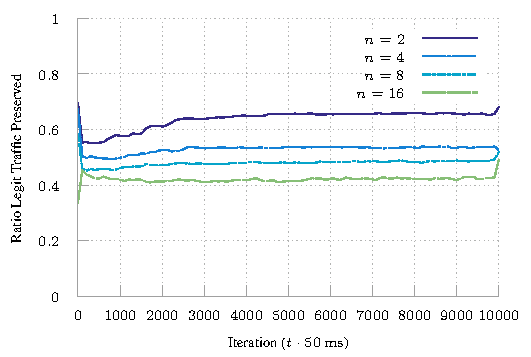
\includegraphics[width=\linewidth]{../plots/online-varyN-binary}
	\caption{
		MARL pushback control system performance plotted over time for various settings of $n$ hosts per agent.
		This plot shows that, from the perspective of benign hosts, service guarantees degrade as inference and actions become less granular.
		This generalises for all behavioural discriminators: even a perfect agent \emph{must} punish benign flows if they are grouped with malicious actors.
		%		?? Effect on max perf AND learning rate??
		Crucially, both the maximum achievable performance and learning rate are negatively impacted when granularity is coarse.
		\label{fig:marl-granularity}
	}
\end{figure}

\Cref{fig:marl-granularity} shows that as more hosts are allocated to each learner, the fraction of traffic believed to be good (as observed at the server) decreases.
This manifests in two ways: the best-achievable performance drops, and so too does the learning rate.
The first consequence arises analytically.
Given the probability that a host is legitimate, $P_G \in [0,1]$, it follows that a host will be malicious with probability $P_B = 1 - P_G$.
Defining \emph{imperfect service} to mean any case where all $n$ hosts connecting over a switch do not share the same classification (i.e., a mixture), then the probability that a switch is delivering imperfect service is $P_{M,n} = 1 - (P_G^n + P_B^n)$.
\begin{thm}
	As $n$ increases, it is more likely that a throttling switch will exhibit imperfect service: $\forall n \in \mathbb{Z}^{+}, P_{M,n} \le P_{M,n+1}$.
\end{thm}
\begin{proof}
	\emph{Base case:} $P_{M,1}=0, P_{M,2} = 1 - P_G^2 - P_B^2 > 0$.
	\emph{Inductive step:} Assume that the theorem holds for $n$. Observe that $P_G^n \ge P_G^{n+1}$ (resp.\ $P_B$). It then follows that:
	\begin{align*}
	P_G^n + P_B^n &\ge P_G^{n+1} + P_B^{n+1}\\
	1 - (P_G^n + P_B^n) &\le 1 - (P_G^{n+1} + P_B^{n+1})\\
	P_{M,n} &\le P_{M,n+1}
	\end{align*}
\end{proof}
\begin{corr}
	Restricting $P_G \in (0,1)$ so that both $P_G$ and $P_B$ are non-zero ensures strict inequality: $P_{M,n} < P_{M,n+1}$.
\end{corr}

%?? Expand according to the summary you posted in the notes document.
%That the use of UDP-like traffic replicates their experiments, compared against how real tcp behaves in mininet and according to the Mathis equation, shows that they really did not consider the behaviour of benign TCP in this environ (i.e., their results should be considerably worse in practice).

\subsection{TCP Multiplexing and Fallback Behaviour}\label{sec:tcp-multiplexing-and-fallback-behaviour}

%While Tcpreplay was useful in recreating the original work and examining the above condition, flow behaviour under packet loss is closer to that of UDP when using it to replay traffic.
%To investigate the effects of collateral damage upon benign TCP flows, an iperf3 test was conducted using mininet.
%Several hosts communicated concurrently to a single server over one switch, with maximum send rates in $\{1,...,5\}$ \si{\mega\bit\per\second} and a constant \SI{40}{\milli\second} latency.
%The rate of packet drop was increased linearly from \SIrange{0}{40}{\percent} and the observed throughput for each host was measured, to show a trend and determine for the mininet environment whether throughput would decrease as expected, at a super-linear rate.

%\begin{figure}
%	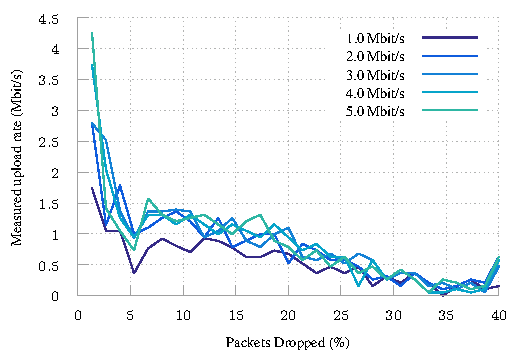
\includegraphics[width=\linewidth]{../plots/mplex}
%	\caption{
%		Average TCP upload rate of hosts targeting different bandwidths in \emph{mininet}, computed over 10 runs, for choices of packet drop rate up until throughput is reduced to almost \SI{0}{\mega\bit\per\second}.
%		As the rate of packet drop increases from \SIrange{0}{40}{\percent}, all flows converge on an extremely low throughput, regardless of the target bandwidth---a super-linear decrease for legitimate TCP traffic.
%		Prior treatments have ignored such phenomena, which have strong implications on agent and network design.
%		Malicious flows are not expected to obey the Mathis equation in this way, worsening collateral damage experienced by benign TCP flows.
%		\label{fig:mplex-tcp}
%	}
%\end{figure}

\begin{figure}
	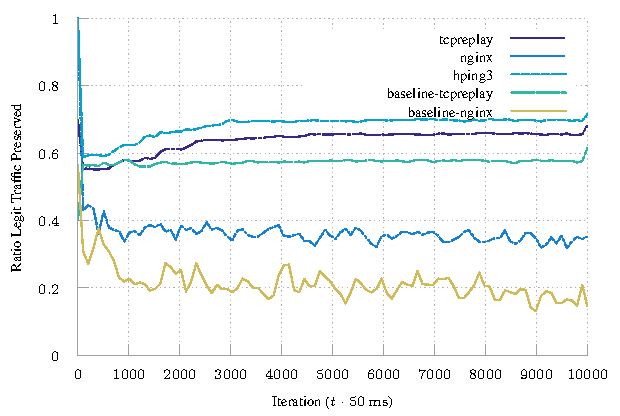
\includegraphics[width=\linewidth]{../plots/online-varyN-nginx}
	\caption{
		Comparison of preserved traffic across different traffic models, choosing $n=2$ hosts per egress node.
		No actions are taken in the ``baseline'' entries.
		The agents examined here perform above the baseline when traffic sources pay no mind to congestion control, but perform significantly worse for live TCP traffic (nginx).
		\label{fig:nginx-coffin-nail}
	}
\end{figure}

%\Cref{fig:mplex-tcp} shows that this trend is present.
Given the UDP-like behaviour of Tcpreplay, being able to replicate the online performance of \citeauthor{DBLP:journals/eaai/MalialisK15} in the $n=2$ case suggests that the numeric simulation their work is entirely based upon does not capture the key interactions between TCP flows and packet drop as a control action.
From the Mathis equation \cite{DBLP:journals/ccr/MathisSMO97}, through which the performance characteristics of TCP under packet drop are well-known and well-understood, their results should be considerably worse in practice:
\begin{equation}
\operatorname{BW} = \frac{\operatorname{MSS}}{\operatorname{RTT}} \frac{C}{\sqrt{p}},
\end{equation}
for the \emph{maximum segment size} (MSS), \emph{round trip time} (RTT), a choice of constant $C \approx{} \sqrt{3/2}$ dependent on system assumptions, and the probability $p \in (0, 1]$ that a packet is lost.
Accordingly, benign TCP flows are severely harmed by \emph{any} packet drop, so collateral damage to these hosts is more significant.
Good-faith TCP congestion avoidance causes these flows to attempt to back off very quickly.
\Cref{fig:nginx-coffin-nail} shows that this trend is present.
%?? Talk about the same major points you made in the presentation here (i.e. TCP interactions) w/ pushback. Or in the evaluation...
The TCP traffic as it appears here is generated according to \Cref{sec:a-new-normal}.
UDP, however, behaves as expected---malicious hosts are expected to exhibit the same behaviour, given that congestion is their primary goal.
As far as future network protocols are concerned, QUIC \cite{DBLP:conf/sigcomm/LangleyRWVKZYKS17}, a congestion-aware stream transmission protocol, will behave much like TCP.

\subsection{Computational Cost}
%?? Consider talking about the execution times of the old MARL approach here? They're real nice (as expected), so we have lots of room to play around with while (hopefully) remaining under the 1ms target time given by \textcite{DBLP:conf/sigcomm/ChenL0L18}.

Measurements during each of these experiments indicated that the cost of computing any action is typically within \SIrange{80}{100}{\micro\second}.
This is reassuring when measured alongside the insights from other work.
\textcite{DBLP:conf/sigcomm/ChenL0L18} observed that, ideally, actions must be computed and taken within \SI{1}{\milli\second} to have a meaningful affect on short flows.
%Most flows are short, and flow-size follows a heavy-tailed distribution.
That our starting point falls significantly below this threshold allows us to safely consider more costly actions or larger state spaces, which would typically increase the computational cost.

%\subsection{Synthesis}
%%It'd be really good if I could figure out a rough proof for the service property...
%%Okay... now say what this means for future viability! What changes can I make? Flow-specific metrics, of course! Increase granularity as much as I can!
%Both of these experiments suggest that the most viable way to enhance and deploy this MARL approach is to consider flows individually to maximise performance for legitimate hosts and to detect malicious hosts in a more principled manner.
%While this will add significant computational cost, this may be worked around with intelligent sampling and monitoring while taking multiple actions per-timestep \cite{DBLP:conf/hotnets/MaoAMK16}.
%
%?? Observations: training time lengthier by nature of emulated environment.
%?? Risk of going for a simulation (i.e. numeric)? Always going to be interesting behaviour that is missed out on (in theory), at the cost of training time/limits of simulation speed

\section{A New Normal}\label{sec:a-new-normal}

%In establishing...
%
%?? How will I structure this?
%?? Motivation -> Model -> Results?
%?? OR Use the results of the last section to springboard into here?

?? Remember, the motivation is clear. We don't care so much that it is "representative" wrt a specific deployment location or network type. The whole purpose of this is that we aim to test specific behaviour which traces cannot replicate (i.e., correlated back-and-forth, dynamics introduced to congestion-aware protocols, ...)
?? If we need to, we can codition the distribution of requests according to statistics mined form an existing trace if reviewer number 2 needs that extra push to be convinced.

?? Full Openflow controller setup (in mininet). All internal routers are primed with knowledge of the shortest path to any internal host, while new inbound flows register the ``way back'' for each hop used to maintain consistency over traffic conditions.
If such information is lost, it suffices to forward an outbound packet on a random (outbound) port, as we assume that any external IP is reachable through any of the test network's egress ports (i.e., that it is not connected to any stub autonomous systems).
The controller is also responsible for responding to ARP traffic, as a gateway might do.
The necessity of this arises due to the realities of relying upon Linux's IP stack, and would not need to be considered for purely trace-based evaluation.
?? Legitimate traffic: TCP traffic (HTTP clients downloading web pages, dependent resources and files) with a mixture of lifetimes for each request.
?? Malicious traffic: UDP flood traffic (hping3, MTU-size packets, ). Why not min-size packets? Because the traffic generator gets in a horrible rut if I do so...

?? Actually describe what I have here, now.

?? ANGLE: set up an environment to test \emph{specific} behaviours to examine \emph{specific} problems in past work. I make no claims that it is perfect or representative for all traffic, just for this (likely common) behaviour which I expect to plague almost all legit TCP flows.

?? Existing sims used for testing such applications reliant on traces, or not sophisticated enough to capture interactive, back-and-forth (correlated) behaviours---possibly discarded as second-hand effects by past work when these are so crucial given user traffic patterns (and the nature of the control signal we choose to enact).

?? Two modes: long-flow (i.e., groundhog day loop of GCC8 download) and nice request-chain mode for ``representativeness''(??)

\section{Rethinking the State Space}\label{sec:rethinking-the-state-space}

?? Mention Colin/Qianru's concerns about Quic, IPv6. At this point, src/dst IP are the only ``traditional'' characteristics that can be relied upon. Even then, IPv6 can have a different IP for each application ON A HOST. Port number meaningless...

?? What do we want?

\textbf{Global state}---what came before (load statistics from various network locations)

\textbf{Local state}---per-flow data. Specifically, right now I'm using:

?? \emph{IP}

?? \emph{Last action taken}: encodes the notion of current belief of flow maliciousness (default at 0). Potentially allows forgiveness: a mistakenly malicious flow 's falloff after punishment could be used for such purpose (if we're lucky...)

?? \emph{Flow duration, size}

?? \emph{Correspondence ratio}: ratio (in bytes) between upstream/downstream traffic for a src/dst pair. (Cite the work that suggested this)

?? \emph{Change in send/recv rates} since last action/check.

?? \emph{Mean inter-arrival time}.

\subsection{What's done with these?}

?? Tile coded together, action taken per-flow every timestep.

?? TODO: everything

?? What concessions will we have to make in order to make per-flow processing more viable? Intelligent sampling/reanalysis of flows when needed (i.e. an external heuristic guiding method)?

?? NOTE: think about how I might need to change/alter the tile-coding when we add extra discriminative features... (i.e., are there better ways to handle covariance between properties of system/flow state, properly capture generalisation?)

?? What might we do for a reward function in the absence of heuristic estimates and/or explicit a priori knowledge? I think a good candidate is the sum of up and down throughputs (normalised by capacity sum), so long as \emph{neither exceeds the link capacity}. We can extend the team-based formulations similarly. This, in theory, promotes traffic diversity since it's not like flooding-based DDoS attacks are going to submit meaningful work to a server. The intuition, I suppose, is that certain classes of flow will have a small footprint in one direction which causes a sizeable increase in the other!

\section{The Results of Doing So}\label{sec:the-results-of-doing-so}

?? They'd probably look real nice...

\section{Related Work}

?? Other recent work in the prevention of DDoS? (i.e., non-RL).
\emph{Athena} \cite{DBLP:conf/dsn/LeeKSPY17} had it as part of their evaluation, BGP-like rerouting techniques (specifically for transit-link attacks, but also for `normal' attacks) \cite{RoutingAroundCongestion}

%?? Abuses of RL 
Earnest, well-considered application of RL towards the challenge of intrusion detection/prevention has seen comparatively little examination.
Past work exhibits treatment of the paradigm as a traditional classifier for anomaly detection \cite{shamshirband2014anomaly} and DDoS prevention \cite{DBLP:conf/mates/ServinK08}.
Given that arguably the main strength of RL techniques is their ability to control ongoing interaction and to adapt by observing the concrete effects of actions taken, such works fail to see how best to apply the rich literature on the subject.

For categorising how RL fits into solving problems, we label works as direct- or indirect-control RL.
A \emph{direct-control} RL problem is one where the RL agent(s) are learning optimal control over a set of actions to act as the \emph{primary} defence or decision-maker---requiring measurements, reward functions and action sets tailored for this purpose.
?? Good Direct-control work? What this work is based on (which directly captures the spirit of RL) \cite{DBLP:phd/ethos/Malialis14, DBLP:journals/eaai/MalialisK15}

An \emph{indirect-control} RL problem, where the role played by the agents is to act in service to \emph{another technique} responsible for decision-making, further optimising or generalising aspects of its operation beyond that of hand-coded heuristics.
%Indirect-control applications: link to all the juicy stuff in e.g. HotNets, data-driven networking, the works. \cite{DBLP:conf/hotnets/ValadarskySST17, DBLP:conf/hotnets/MaoAMK16}.
A past example includes learning when best to \emph{communicate} and share knowledge between \emph{hidden Markov model} anomaly detectors \cite{DBLP:conf/paisi/XuSH07}.
The position of this work is weakened by its reliance on the discredited `DARPA99' dataset \cite{DARPA-IDD, DBLP:conf/cisda/TavallaeeBLG09, DBLP:conf/sp/SommerP10}, but the idea itself is well-treated and this acts as a driver for improvements in this direction.
Outside of anomaly/intrusion detection, there has been growing interest in the use of reinforcement learning in data-driven networking, such as for intra-AS route optimisation \cite{DBLP:conf/hotnets/ValadarskySST17} and for resource-constrained process allocation \cite{DBLP:conf/hotnets/MaoAMK16}.
?? Also adaptively choosing video bitrates based on network conditions \cite{DBLP:conf/sigcomm/MaoNA17}.

?? Completely reword, yikes.
\citeauthor{DBLP:conf/sigcomm/ChenL0L18}'s \emph{AuTO} \cite{DBLP:conf/sigcomm/ChenL0L18} uses deep RL (the \emph{deterministic policy gradients} algorithm \cite{DBLP:conf/icml/SilverLHDWR14}).
Crucially, they find that decisions need to be made for the vast majority of (short-lived) flows, sub-millisecond.
Their work falls between the above two paradigms: to overcome the high latency of action computation via neural network, two agents are trained.
The first learns to optimise flow size thresholds governing priority (and accordingly demarcate long and short flows).
All short flows are routed by ECMP.
The second agent makes decisions about routing, prioritisation etc.\ for these long flows, who are likely to live long enough that any decisions made will have a significant impact.

These works emphasise the necessity of ingenuity in effectively handling how states and actions are represented.

\section{Conclusion}

It all ends here...

?? Please write me once everything else is in place.

?? Future Work? I.e., \emph{everything}: no one else is really looking at/interested in this specific kind of application of RL yet. \emph{Yet}.

?? IDEA: try out average reward, TD($\lambda$) methods as future work...

?? IDEA: Apply these techniques to programmable data planes etc. While it's pretty neat that what we have works assuming that ach router is a software (x86) switch running OVS, what might we need to consider when applying this to `real' switches? ``PDP can allow this to be added to real routers to make it efficient to keep \& process state in the manner we require, as well as enabling more adaptive deployment''. Cite P4, BPFabric, other work on PDPs?

?? Benefit of the more realistic emulation environment is that it is far closer in behaviour and architecture (i.e. viable) to a real SDN-enabled deployment, captures some dynamics which were otherwise hidden/lost by human ignorance. It also allows me to develop the system towards evolving traffic models where it is expected that RL should shine over and above standard ML techniques. THEN: Room to introduce/roll-in dynamic changepoint detection or adaptive exploration \cite{DBLP:conf/ki/Tokic10, DBLP:conf/ki/TokicP11, DBLP:conf/annpr/TokicP12}?

?? Overarching goal: works which \emph{respect the complexity of the network environment} (rather than na\"{i}ve simulation, blind ML applications etc.) and choose well-considered pathways to solution. \emph{Call-to-action}?

?? Security? I suspect that the very qualities that make inference difficult in IDS/IPS also increase the level of challenge an advanced threat must overcome.
System state which is dependent on many signals drawn from across a wide network, in concert with their burstiness and unpredictability, may have substantial effects on an attacker's capabilities.
?? Might want to mention it in related work above, but the recent attention on adversarial examples/tricking models needs to be looked into for RL. Poisoning attacks relevant for online techniques: old bounds exist \textcite{DBLP:journals/jmlr/KloftL10}, new stuff concerns collaborative learners \cite{DBLP:conf/acsac/ShenTS16}, nothing for rl. Hot topic in deep networks \cite{DBLP:conf/eurosp/PapernotMJFCS16, DBLP:conf/eurosp/PapernotMSW18}, but naturally still relevant with even linear approximations or exact tabular case due to limits of the PAC assumption. There is now examination of evasion attacks wrt.\ RL \cite{DBLP:journals/corr/HuangPGDA17}!
?? evasion attacks by \textcite{DBLP:conf/sp/Carlini017}---all of these are computed by way of a general stochastic optimiser, such as \emph{Adam} \cite{DBLP:journals/corr/KingmaB14}. possible to apply something similar to our learned model to assess its security? would the suggested states even be valid? (i.e. since they're monotonically increasing for the most part).

?? More future work --- share knowledge between agents. ``Knowledge bases'' for this purpose? (see: Qianru).

\section*{Acknowledgements}
My thanks go to Mircea Iordache, Qianru Zhou, and Richard Cziva for their comments and technical assistance.
Additional thanks \emph{would} go out to my anonymous reviewers, had I any of them.

\renewcommand*{\bibfont}{\small}
\printbibliography

\end{document}